\documentclass[11pt]{book}


% Be sure to use PDF Latex
\pdfoutput=1


% links
\usepackage[bookmarks,bookmarksdepth=2, colorlinks=true, linkcolor=blue,citecolor=red, urlcolor=blue]{hyperref}


\usepackage{fullpage}

\usepackage[utf8]{inputenc}
% \usepackage[latin1]{inputenc}
\usepackage[french]{babel}

\usepackage{mystyle}
\renewcommand{\guill}[1]{«~#1~»} % french

\usepackage{url}

\usepackage[T1]{fontenc}

%\usepackage{vmargin} \setpapersize{A4}
%\newcommand{\mypage}{30mm}
% \setmarginsrb{\mypage{}}{\mypage{}}{\mypage{}}{\mypage{}}{0mm}{0mm}{0mm}{0mm}

\graphicspath{{./figures-nn/}}
\newcommand{\otarticle}

\title{Les mathématiques des réseaux de neurones} 

\author{%
\begin{tabular}{c}
	Gabriel Peyr{\'e} \\ CNRS \& DMA \\
	 PSL, \'Ecole Normale Sup\'erieure \\
	 \url{gabriel.peyre@ens.fr}
\end{tabular}
}
\date{}

\begin{document}

\maketitle

%%%%%%%%%%%%%%%%%%%%%%%%%%%%%%%%%%%%%%%
\chapter{Les réseaux discriminatifs}
Since 2012, deep neural networks have revolutionized machine learning.
%
Although relatively old, in recent years this technique has allowed very spectacular advances in the recognition of texts, sounds, images and videos.
%
Understanding the stakes of these methods raises questions at the interfaces between mathematics and algorithmics.
%
In this article, I will explain the structure of these networks as well as the key concepts of their supervised learning.
% !TEX root = ../NeuralNetworksEN.tex

%%%%%%%%%%%%%%%%%%%%%%%%%%%%%%%%%%%%%%%%%%%%%%%%%%%%%%%%%%
%%%%%%%%%%%%%%%%%%%%%%%%%%%%%%%%%%%%%%%%%%%%%%%%%%%%%%%%%%
\section{Algorithmics and mathematics of learning}

Neural networks are algorithms, which compute, from an input $\myblue{x}$ (for example an image), an output ${\color{red} y}$. As shown in figure~\ref{fig:discriminative}, this output is most often a set of probabilities: for example the first output is the probability that the image contains a cat (the closer this number is to $100\%$, the more it means that the algorithm is sure of itself), the second is the probability that the image contains a dog, etc.
%
To simplify, we will consider in our examples only two classes: cats and dogs, but in practice one can consider an output ${\color{red} y}$ with several thousands of classes. We also restrict ourselves to the example of images, but neural networks are also very efficient in recognizing texts or videos.

Mathematically, such an algorithm defines a function $f_{\mygreen{w}}$ (i.e. ${\color{red} y} = f_{\mygreen{w}}({\color{blue}x})$). The computer program that calculates this function is very simple: it is made up of a sequence of several stages, and each stage performs elementary calculations (additions, multiplications, and a maximum).
%
In comparison, the computer programs found in a computer's operating system are much more complex.
%
But what makes the huge difference between a \guill{classical} algorithm and a neural network is that the latter depends on parameters, which are the weights of the neurons. Before using a neural network, these weights must be modified so that the algorithm can best solve the requested task. This is done using mathematical and algorithmic methods which will be explained in the following sections. This process is called \guill{training} a neural network, and this requires a lot of time, machine calculations and energy.

Using these algorithms wisely therefore requires computer science and mathematics skills. It is thus necessary to manipulate  key concepts in computer science (iterative methods, computation time, memory space, efficient implementation, \ldots) and mathematics (linear algebra, optimization, statistics, \ldots).

%%%%%%%%%%%%%%%%%%%%%%%%%%%%%%%%%%%%%%%%%%%%%%%%%%%%%%%%%%

\section{Discriminative neural networks}

An artificial neural network is built around a biological metaphor.
%
The structure of the primary visual cortex is relatively well known, and Hubel and Wiesel won the Nobel Prize in Physiology for the discovery in 1962 of the organization of neurons in the first cortical layers~\cite{hubel1962receptive}.
%
Thus, in an extremely simplified view of the brain, neurons are organized in layers, each neuron retrieves information from a previous layer, performs a very simple calculation, and communicates its result to neurons in the next layer.
%
It must however be keep in mind that this is only a metaphor and a source of inspiration: biological networks have much more complex connections and the mathematical equations which govern them are also more complex (they have been discovered by Alan Hodgkin and Andrew Huxley in 1952~\cite{hodgkin1952quantitative} and they won the Nobel Prize for this).
%
It therefore remains difficult to precisely relate the sometimes surprising performances of artificial neurons to the cognitive capacities of the brain. For example, the techniques to train artificial networks which I will now explain are quite different from the way a child learns.

\begin{figure}\centering
	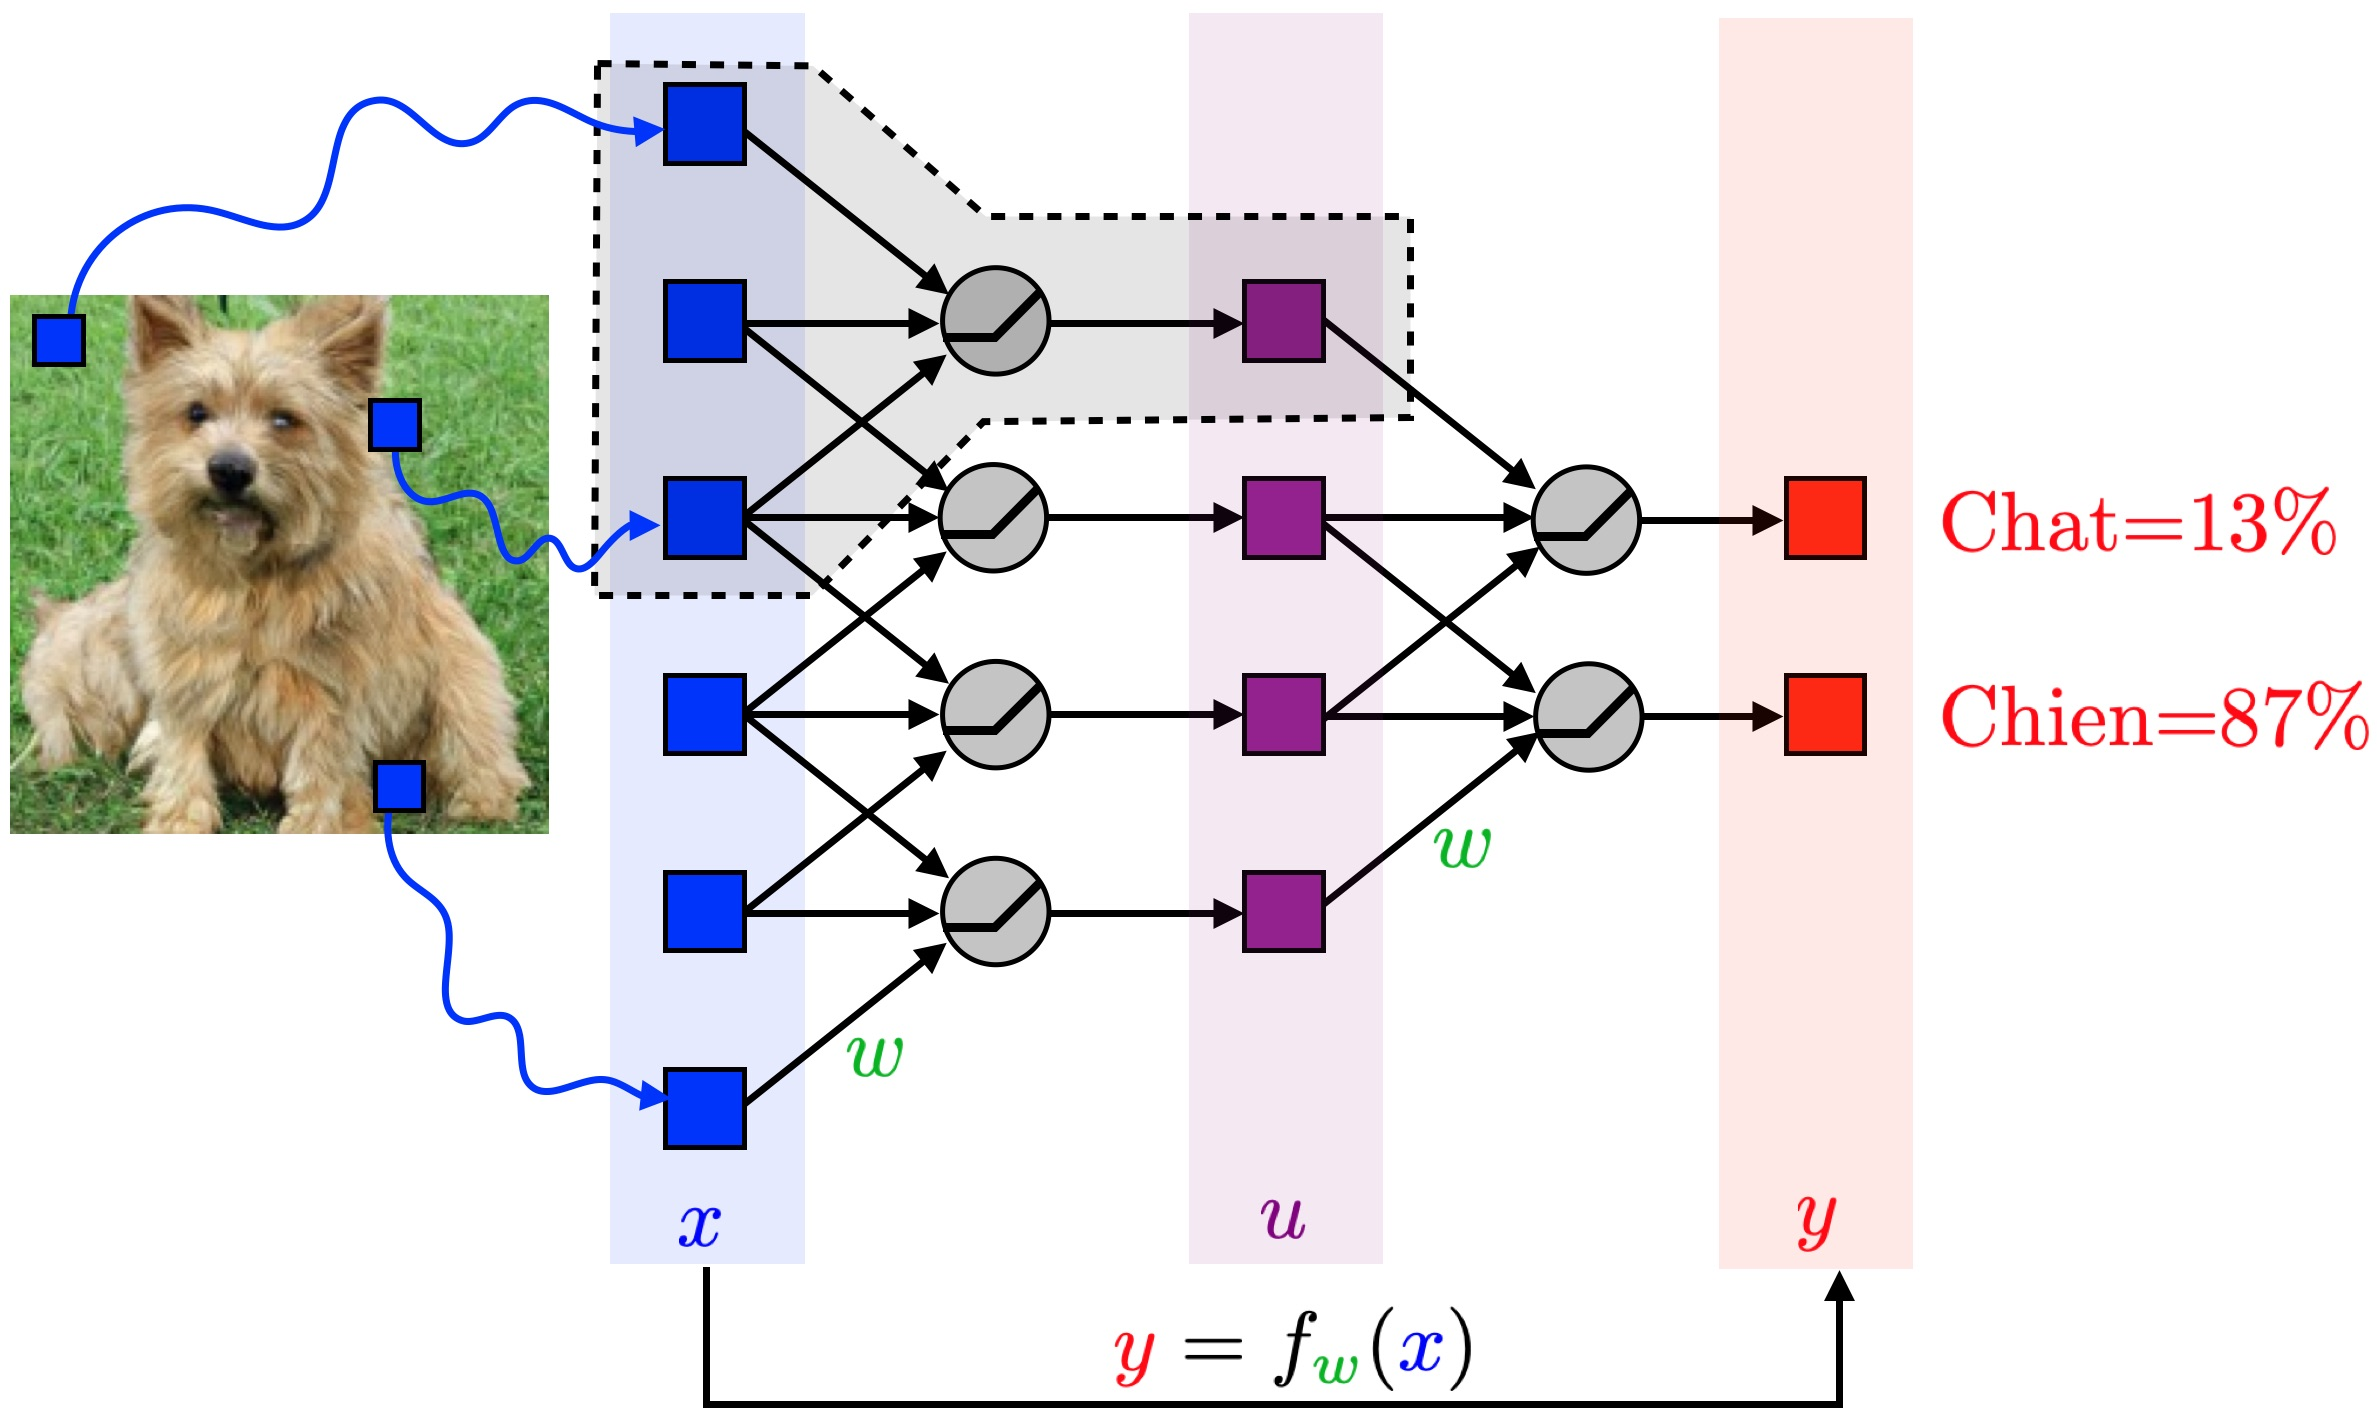
\includegraphics[width=.8\linewidth]{discriminative}
\caption{\label{fig:discriminative} 
Example of a discriminative neural network with two layers.  }
\end{figure}

Figure~\ref{fig:discriminative} details an example of such an artificial network.
%
This type of neuron was introduced in 1943 by McCulloch and Pitts~\cite{mcculloch1943logical}.
%
To simplify, it is here composed of only two layers of neurons (the first layer between ${\color{blue} x}$ and ${\color[rgb]{.5,0, .5} u}$, the second between ${\color[rgb]{.5,0,.5} u}$ and ${\color{red} y}$), but today's most efficient networks can have several dozen layers, we say that they are deeper.
%
In our example, the inputs ${\color{blue} x}$ are the pixels of an image. An image typically contains millions of pixels, and the figure voluntarily represents only a small number: a realistic network is indeed more complex. In addition, each pixel that makes up ${\color{blue} x}$ is actually made up of 3 values (one for each primary color red, green and blue).

Passing from one layer (for example the ${\color{blue} x}$ layer of inputs) to another (for example the second layer ${\color[rgb]{.5,0,.5} u}$, which is a \guill{hidden} layer in the middle of the network) is done through a set of artificial neurons. A neuron is represented on the figure~\ref{fig:neuron}. It is the first neuron, the one that calculates the first value ${\color[rgb]{.5,0,.5} u_1}$ which composes the layer ${\color[rgb]{.5,0,.5} u}$. This neuron connects a certain number of elements of the first layer (here three: ${\color{blue} x_1, x_2, x_3}$, but there can be more) to a single element of the second, so here ${\color[rgb]{.5,0,.5} u_1}$. The formula calculated by the neuron is
$$
	{\color[rgb]{.5,0,.5} u_1} = \max( \mygreen{w_1} \times \myblue{x_1} + \mygreen{w_2} \times \myblue{x_2} + \mygreen{w_3} \times \myblue{x_3} + \mygreen{w_4}, 0).
$$
The neuron thus performs a weighted sum of the three inputs, with three weights $\mygreen{w_1}, \mygreen{w_2}, \mygreen{w_3}$, and we also add $\mygreen{w_4}$, which is a bias. Then the neuron calculates the maximum between this sum and zero. One can also use a function other than the maximum function, but this one is the most popular. It is a thresholding operation. We can compare it to biological neurons which let or not pass information according to whether they are sufficiently excited or not.
%
So if the weighted sum $\mygreen{w_1} {\color{blue} x_1} + \mygreen{w_2} {\color{blue} x_2} + \mygreen{w_3} {\color{blue} x_3} + \mygreen{w_4}$ is smaller than 0, then the neuron returns the value ${\color[rgb]{.5,0,.5} u_1} = 0$, otherwise it returns the value of this sum and places it in ${\color[rgb]{.5,0,.5} u_1}$.


\begin{figure}\centering
	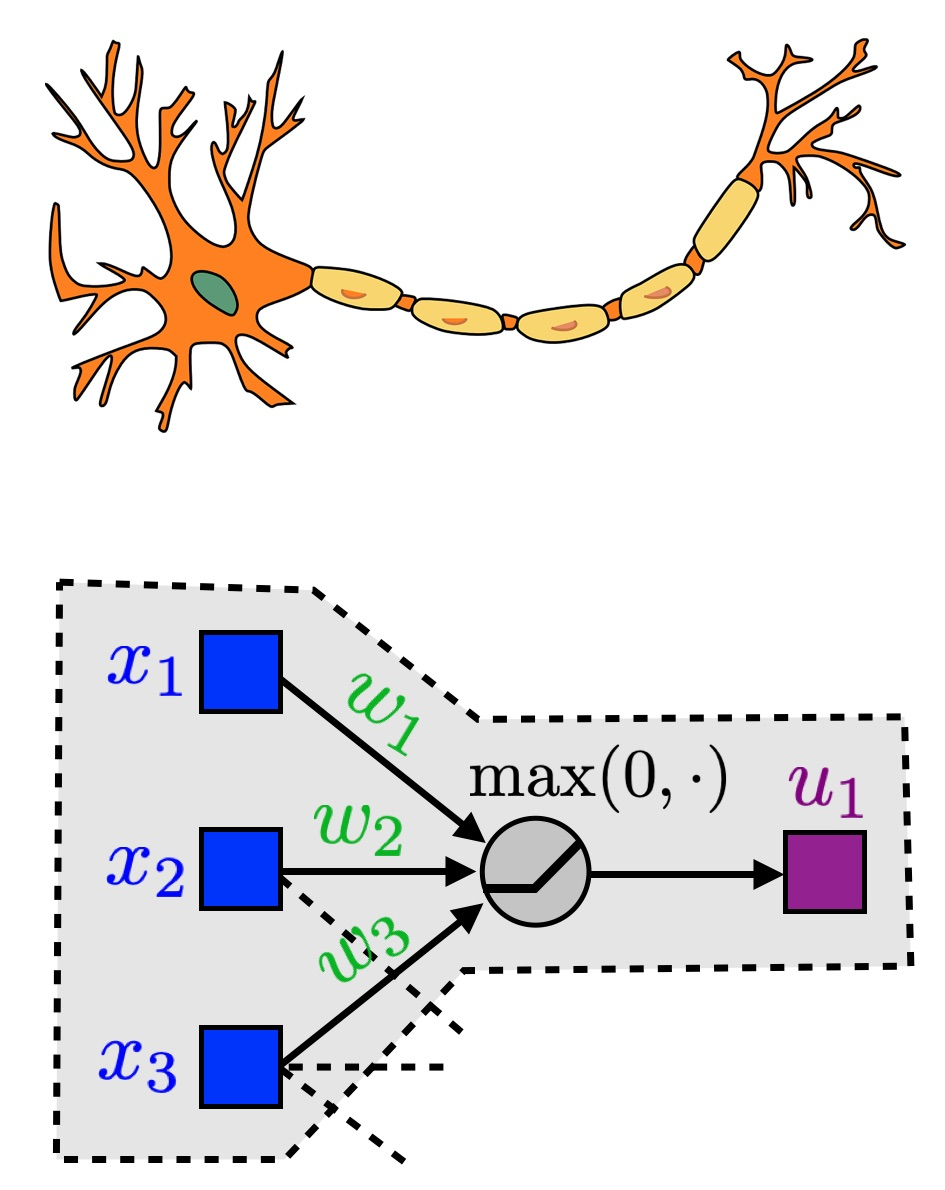
\includegraphics[width=.35\linewidth]{neuron}
\caption{\label{fig:neuron} Biological and artificial neurons. }
\end{figure}

Such neural networks were introduced by Rosenblatt~\cite{rosenblatt1957perceptron} in 1957, who called them \guill{perceptrons}. The first perceptrons contained only one layer.
%
% They were then popularized by the book by Minsky and Papert~\cite{minsky1969perceptrons}.
%
Such single-layer architectures are too simple to be able to perform complex tasks. It is by adding several layers that we can calculate more complex functions.
%
Deep neural networks thus use a very large number of layers. In recent years, these architectures have made it possible to obtain very impressive results for the recognition of images and videos as well as for the automatic translation of texts. It was this research on deep networks that enabled French researcher Yann Le Cun as well as Geoffrey Hinton and Yoshua Bengio~\cite{lecun2015deep} to obtain the Turing Prize in 2019. This prize is considered to be the equivalent of the Nobel Prize in computer science.
%
To get a better understanding of the behavior of these multi-layered networks, one can use the interactive application \url{https://playground.tensorflow.org}.

%%%%%%%%%%%%%%%%%%%%%%%%%%%%%%%%%%%%%%%%%%%%%%%%%%%%%%%%%%
\section{Supervised learning of a neural network}

Training a neural network consists in choosing the \guill{best} possible weights of the set of neurons that make up a network (for example in particular the weights $\mygreen{w_1, w_2}$ and $\mygreen{w_3}$ of the neuron shown in figure~\ref{fig:neuron}).
%
It is thus necessary to choose the values of these weights in order to best solve the task studied on a set of training data.
%
For the recognition of objects in images, this is a supervised learning problem: we have both images ${\color{blue} x}$ and the associated ${\color{red} y}$ (the probability of the presence of a cat and/or a dog in the image).
%
Figure~\ref{fig:dataset} shows some examples of images used to train a network, for which we know what they contain (the class of cats and the class of dogs).
%
It is therefore necessary, before the learning phase, that humans do a long and tedious job of labeling thousands or even millions of images.


\begin{figure}\centering
	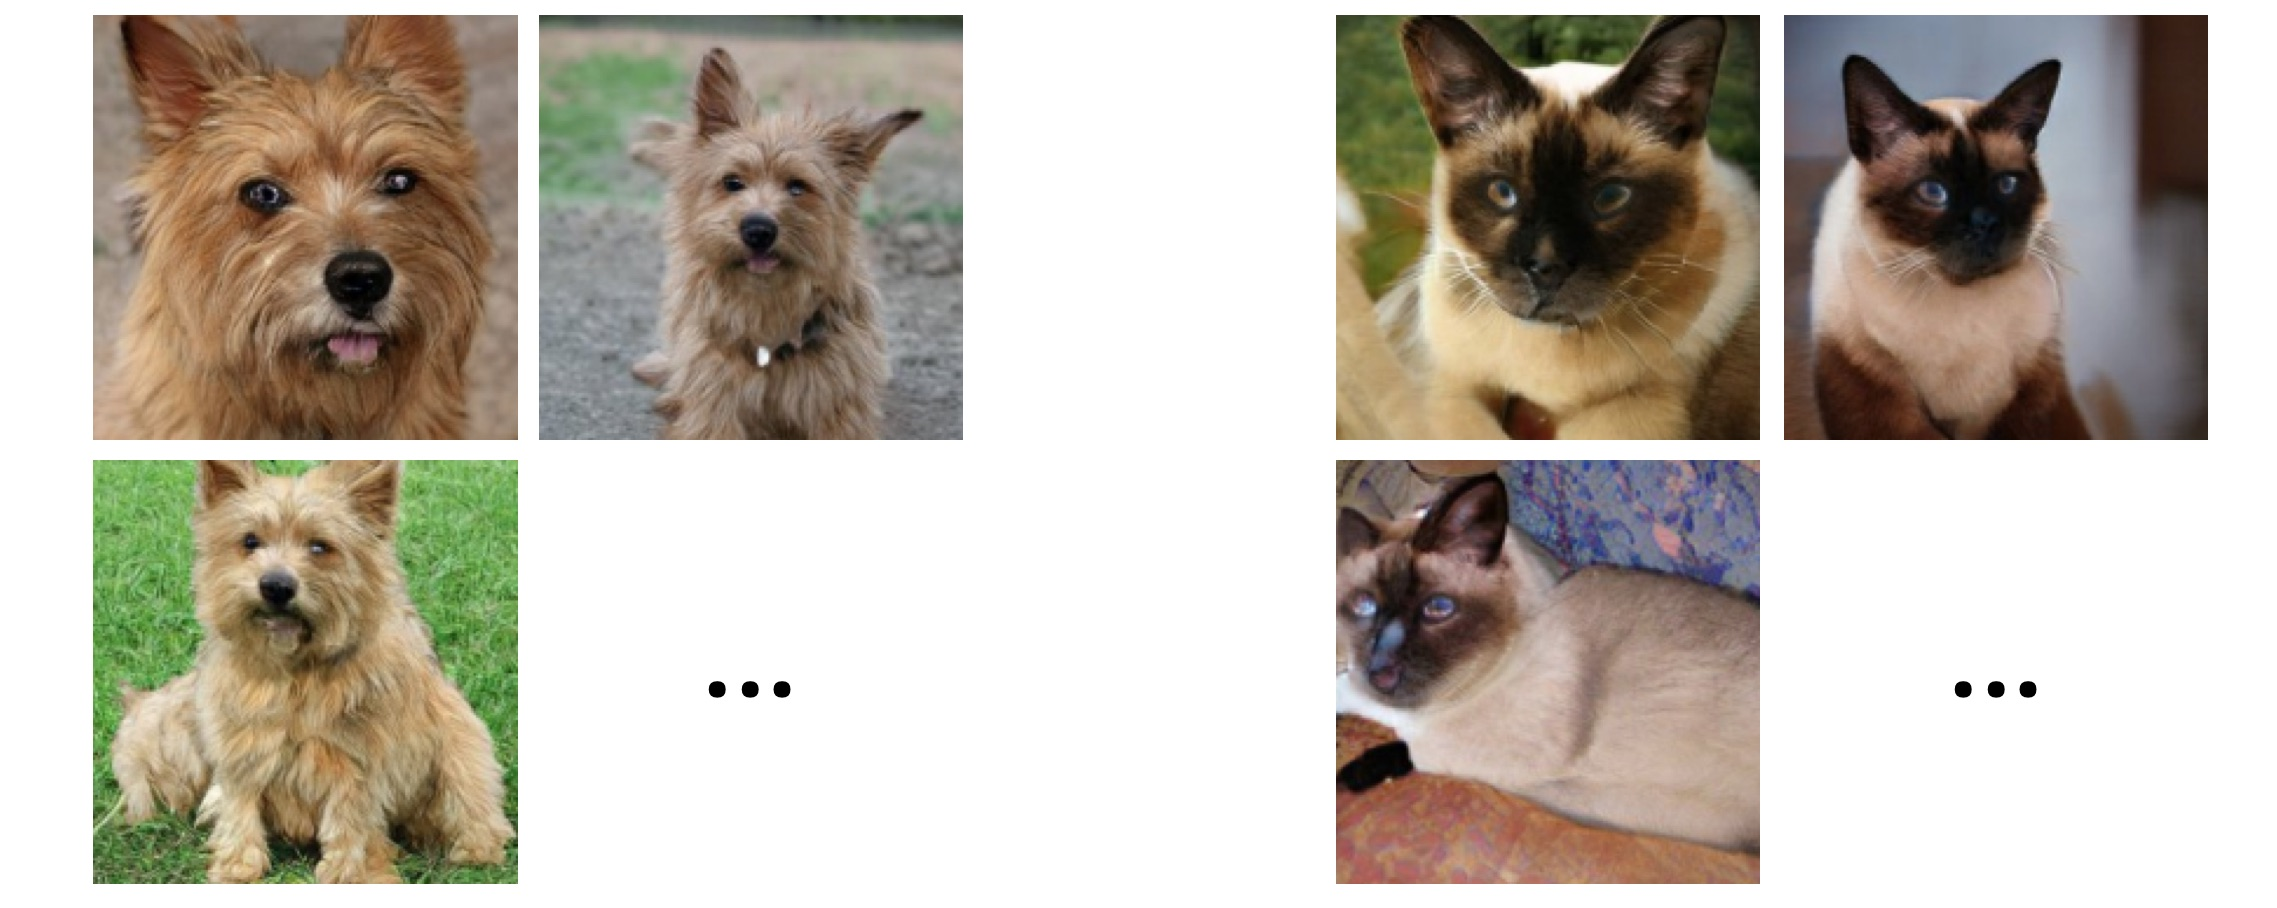
\includegraphics[width=.8\linewidth]{dataset}
\caption{\label{fig:dataset} 
Examples of images from the ImageNet database~\cite{deng2009imagenet} used for learning. }
\end{figure}

The training procedure thus consists in modifying the weights $\mygreen{w}$ such that for each ${\color{blue} x}$, the network $f_{\mygreen{w}}$ predicts as precisely as possible the ${\color{red} y}$ associated, that is to say at the end of the training that ${\color{red} y} \approx f_{\mygreen{w}}({\color{blue} x})$.
%
A simple choice is to minimize the sum $E(\mygreen{w})$ of the squares of the errors, which we write mathematically as
$$
	\min_{\mygreen{w}} E(\mygreen{w}) = \sum_{({\color{blue} x}, {\color{red} y})} (f_{\mygreen{w}}({\color{blue} x}) - {\color{red} y})^2.
$$
%
This corresponds to an optimization problem, because it is necessary to find a set of parameters which optimizes a certain quantity of interest.
%
This is a difficult problem, because there are a lot of parameters, and these parameters, especially those of the hidden layers, have a complicated influence on the result.
%
Fortunately, there are efficient mathematical and algorithmic methods to solve efficiently this type of optimization problem. They are not yet fully understood on a theoretical level and it is a very active area of research.
%
These optimization methods modify the weights $\mygreen{w}$ of the network to improve it and reduce the training error $E(\mygreen{w})$. The mathematical rule for deciding on the weight update strategy is called back propagation~\cite{rumelhart1986learning} and is a marvel of ingenuity, it is a special case of a mathematical and algorithmic method which is called backwards automatic differentiation~\cite{linnainmaa1976taylor}.

These supervised learning techniques date mainly from the 1980s. But it was only in 2012 that a paper by Krizhevsky, Sutskever and Hinton~\cite{krizhevsky2012imagenet} created a tsunami by showing that deep networks can solve complex image recognition tasks.
%
This revolution was possible thanks to the combination of three ingredients: new databases much larger than before~\cite{deng2009imagenet} ; high computing power thanks to graphical processors (\guill{GPUs}, which were previously confined to video games) ; the introduction of several optimization techniques that improve and stabilize learning~\cite{srivastava2014dropout}. 


%%%%%%%%%%%%%%%%%%%%%%%%%%%%%%%%%%%%%%%%%%%%%%%%%%%%%%%%%%
\section{The efficiency of neural networks}

George Cybenko proved in 1989~\cite{cybenko1989approximation} that a neural network$f_{\mygreen{w}}$ with two layers can approximate as precisely as one wants any continuous function $f^\star$ (so in some sense, it can  solve any task, represented by the unknown function $f^\star$, which would be able to recognize objects in any image) as long as the size of the inner layer ${\color[rgb]{.5,0,.5} u}$ (so the number of neurons) is arbitrarily large.
%
This does not mean that such a network $f_{\mygreen{w}}$ with only two layers works well in practice. To apply Cybenko's theorem, it is necessary to have a potentially infinite number of training data, which is far from being the case in practice. 
%
The ultimate goal of learning is not to minimize the learning error $E(\mygreen{w})$, but to be able to predict as precisely as possible a new data. With only a limited amount of data, one will not be able to learn precisely enough, and therefore future predictions on unseen data will be bad. The function $f_{\mygreen{w}}$ will actually be very far from the ideal function $f^\star$ that one would like to learn. 

In order to make the best possible predictions with a limited number of training data, we are therefore looking for the most suitable network architectures, which can efficiently capture the information present in the data.
%
Deep neural networks (with many layers) but with relatively few connections between layers have proven to be very effective on very \guill{structured} data such as text, sound and images.
%
For example, for an image, the pixels have neighborhood relationships, and one can impose specific connections (an architecture) and not connect a neuron with all the others but only with its neighbors (otherwise there would be too many connections). In addition, one can impose that the weights associated with a neuron are the same as those associated with another neuron. This type of networks is called convolutional networks~\cite{lecun1998gradient}.
%
For the moment, there is no mathematical analysis which explains this efficiency of deep convolutional networks. There is therefore a need for new mathematical advances to understand the behaviors and limitations of these deep networks.



%%%%%%%%%%%%%%%%%%%%%%%%%%%%%%%%%%%%%%%
\chapter{Les réseaux génératifs}
Dans l'article précédent, nous avons vu comment entrainer de façon supervisée des réseaux de neurones. Ceci permet de résoudre efficacement des problèmes de classification, par exemple de reconnaissance d'images.  
%
Ce qui est peut être encore plus surprenant, c'est que ces réseaux de neurones sont également utilisés de façon non-supervisée afin de générer automatiquement des textes ou des images \guill{virtuelles}, ce que l'on appelle souvent des \guill{deep fakes}.
%
Dans ce second article, je tisserai un lien entre l'apprentissage de réseaux de neurones génératifs et la théorie du transport optimal. Ce problème a été posé par Gaspard Monge au 18$^e$ siècle, puis il a été reformulé par Leonid Kantorovitch au milieu du 20$^e$ siècle. Il est maintenant devenu un outil de choix pour aborder l'explosion récente de la science des données. 
%
% Le transport optimal est un problème très ancien, formulé par Monge au 18$^e$ siècle. Il a cependant fallu plusieurs révolutions mathématiques pour qu'il devienne un outil incontournable à la fois en théorie et en pratique, jusqu'à son utilisation récente en apprentissage machine.  
% 
% Cet article retrace ces révolutions, initiées par Leonid Kantorovitch pendant la seconde guerre mondiale. La formulation qu'il a proposée se prête à une analyse mathématique poussée ainsi qu'à son application à de nombreux problèmes. Elle fait du transport optimal un outil de choix pour aborder l'explosion récente de la science des données. 
% !TEX root = ../NeuralNetworksFR.tex


%%%%%%%%%%%%%%%%%%%%%%%%%%%%%%%%%%%%%%%%%%%%%%%%%%%%%%%%%%
\section{Réseaux de neurones génératifs}

Au lieu d'utiliser des réseaux de neurones pour analyser des images, des travaux de 2014~\cite{goodfellow2014generative} ont montré qu'on pouvait les utiliser \guill{à l'envers} afin de générer des images.
%
Ces réseaux de neurones génératifs trouvent par exemple des applications pour les effets spéciaux, les jeux vidéo et la création artistique. 
%
On retrouve des questions similaires dans l'apprentissage des voitures autonomes et la résolution de jeux de stratégie.
%
La figure~\ref{fig:generative} montre la structure d'un tel réseau $g_{\mygreen{w}}$, qui dépend de poids $\mygreen{w}$. Les couches jouent en quelque sorte des rôles miroirs par rapport à l'architecture des réseaux de neurones discriminatifs exposés dans l'article précédent.
%
A partir d'une entrée ${\color{red}y}$ composée d'un petit nombre de valeurs, qui sont typiquement tirées aléatoirement, on génère une image ${\color{blue} x} = g_{\mygreen{w}}({\color{red}y})$. 

\begin{figure}\centering
	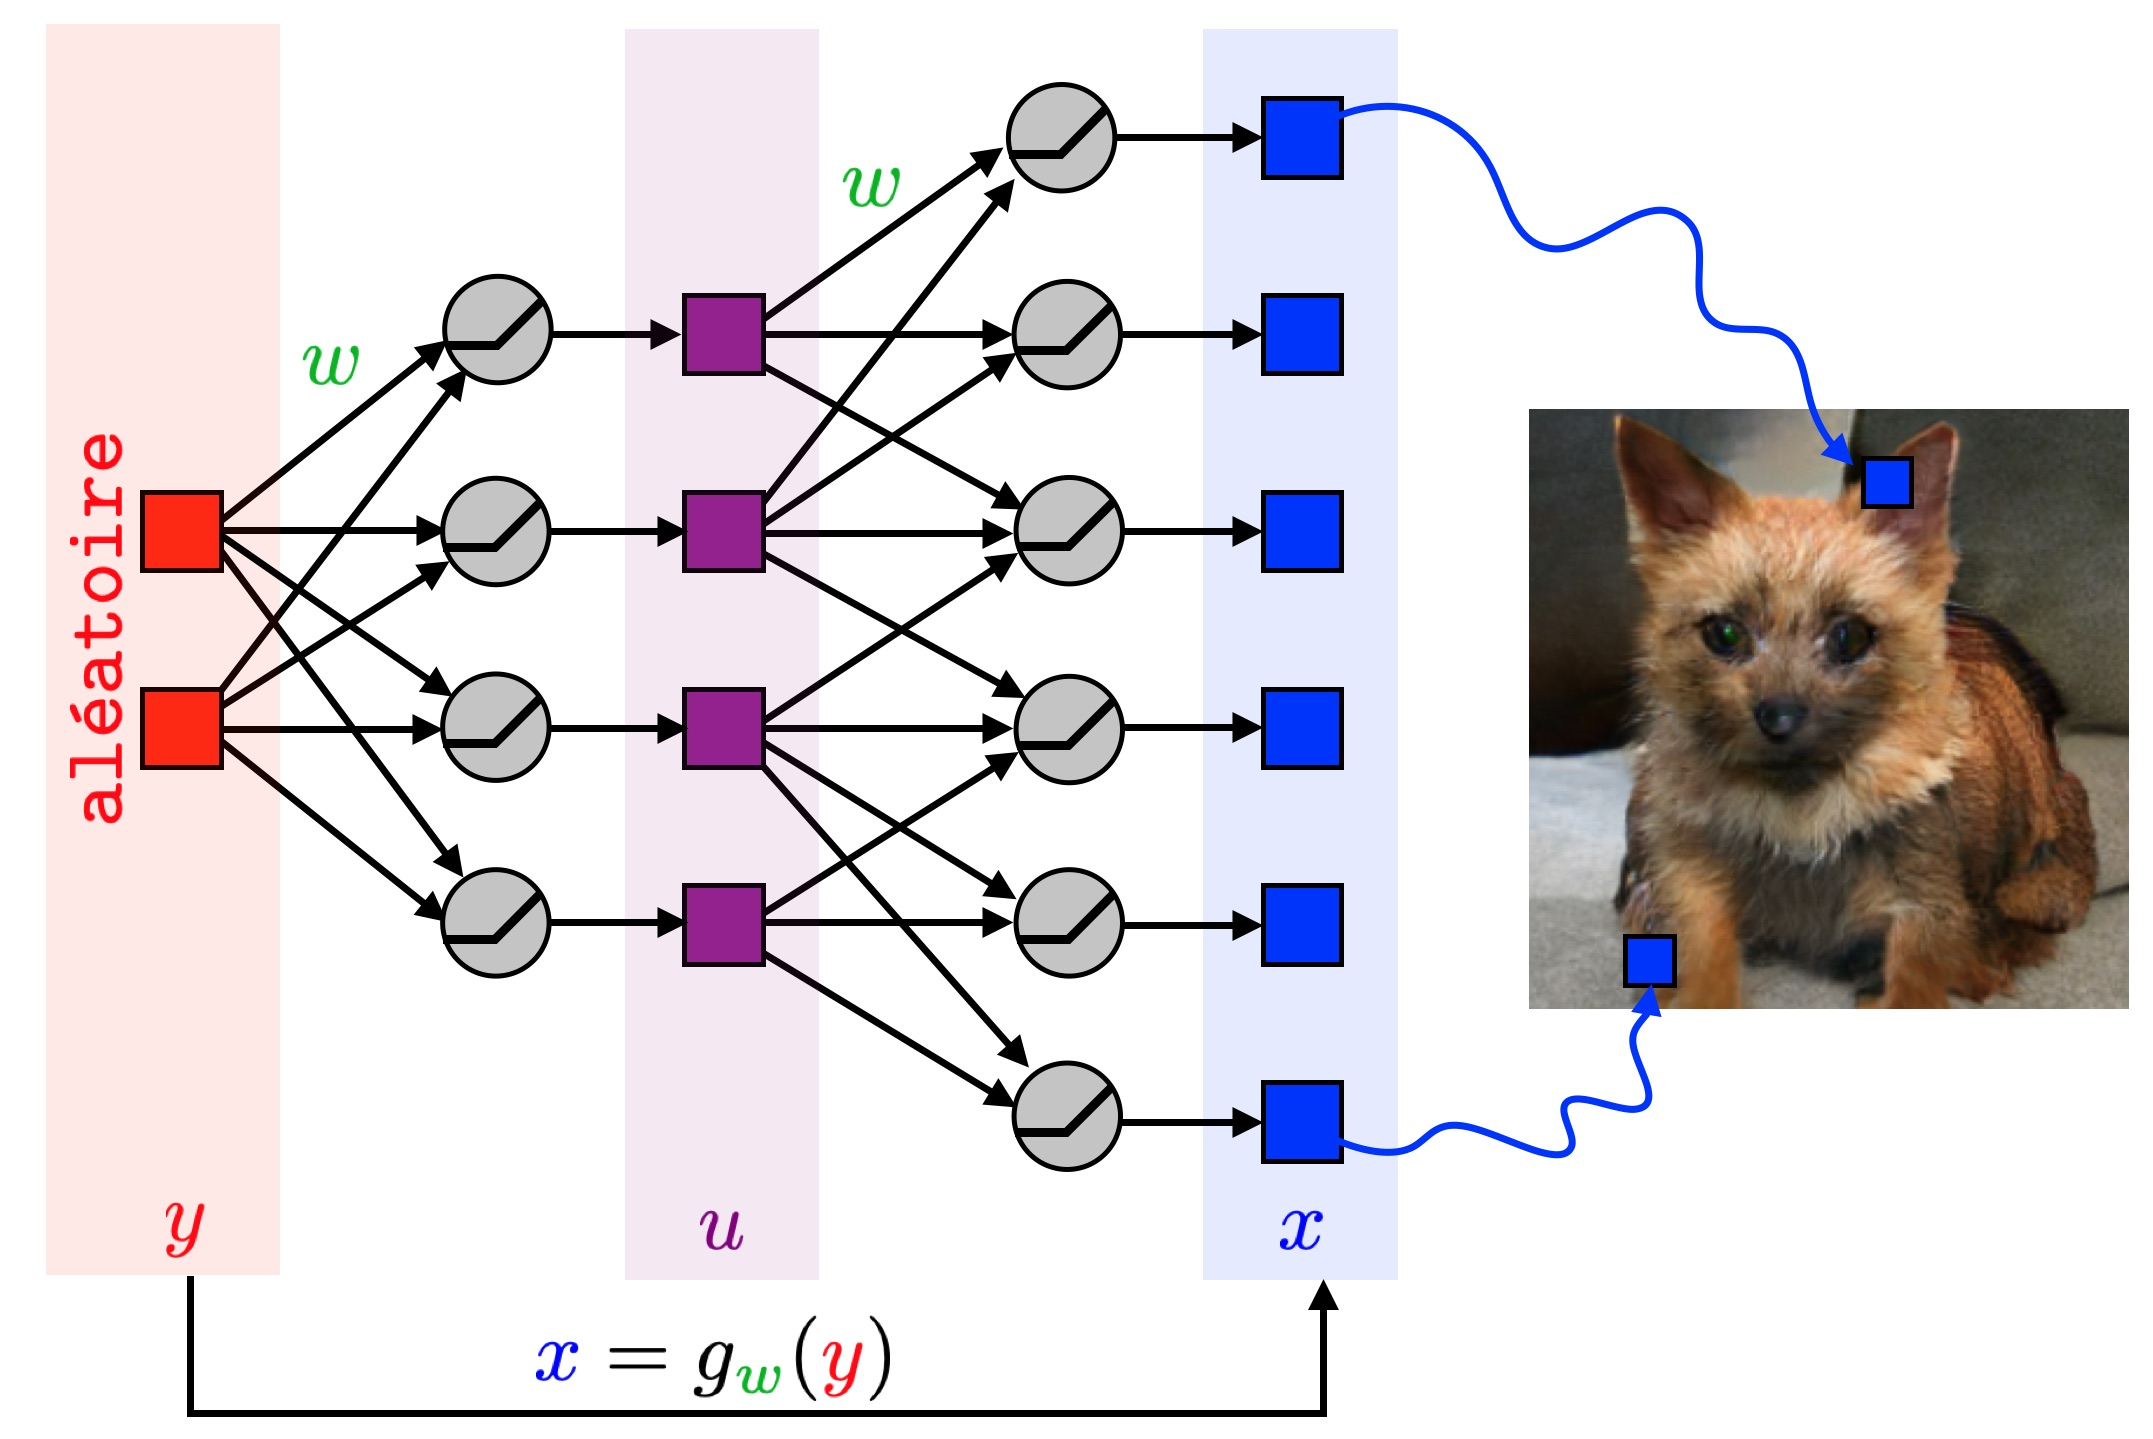
\includegraphics[width=.8\linewidth]{generative}
\caption{\label{fig:generative} Exemple d'un réseau de neurones génératif simplifié (un réseau permettant de générer des images aussi complexes possède plus de couches).  }
\end{figure}

Le problème d'apprentissage de tels réseaux est non-supervisé : on dispose uniquement d'un grand nombre d'images d'apprentissage, sans indication sur ce qu'elles contiennent.
%
Il n'y a plus besoin d'intervention humaine pour indiquer au réseau le contenu des images qu'il doit reconnaitre. 
La collecte de données est ainsi plus simple que pour l'entrainement de réseaux discriminatifs. De plus, ce principe d'apprentissage non supervisé est proche de la façon dont les enfants apprennent, principalement en observant et manipulant le monde qui les entoure.
%
Le but est alors de sélectionner les poids $\mygreen{w}$ des neurones du réseau $g_\mygreen{w}$ de sorte que les images aléatoires générées (les images fausses, \guill{fakes} en anglais) ressemblent le plus possible aux images d'apprentissage. 

%%%%%%%%%%%%%%%%%%%%%%%%%%%%%%%%%%%%%%%%%%%%%%%%%%%%%%%%%%
\section{L'apprentissage non supervisé de réseaux génératifs}
\label{sec-app-gen}

Le but des réseaux de neurones génératifs n'est pas de résoudre une tâche telle que la reconnaissance d'objets dans les images. 
%
Afin d'entrainer les poids $\mygreen{w}$ du réseau, il faut formaliser mathématiquement le problème. Il s'agit de générer un ensemble d'images \guill{virtuelles} (les fausses) qui ressemblent aux images réelles d'une base de données. Il ne s'agit pas simplement qu'une image générée ressemble à une image réelle, il faut mettre en correspondance les deux ensembles d'images. Par exemple, si dans la base de données il y a la moitié d'images de chiens et la moitié d'images de chats, il faut que le réseau génère également pour moitié des chiens et pour moitié des chats. 

On va noter $\{\mylblue{z_1,z_2,\ldots,z_n}\}$ l'ensemble des $n$ images de la base de données. Le nombre $n$ d'images est très grand, de l'ordre de plusieurs milliers ou millions. Etant donné un réseau de neurones génératif $g_{\mygreen{w}}$, qui est paramètré par ses poids $\mygreen{w}$, on note $\{\myblue{x_1,x_2,\ldots,x_n}\}$ un ensemble de $n$ images \guill{fausses} générées aléatoirement par le réseau. Pour générer la première image fausse $\mylblue{x_1}$, ceci signifie que l'on tire aléatoirement les valeurs d'entrée ${\color{red}y_1}$ et qu'on applique le réseau à ces entrées, pour obtenir l'image virtuelle $\mylblue{x_1} = g_{\mygreen{w}}({\color{red}y_1})$. On a ensuite fait la même chose avec $\mylblue{x_2} = g_{\mygreen{w}}({\color{red}y_2})$ et ainsi de suite. 

Le but de l'apprentissage non supervisé est donc de trouver des poids $\mygreen{w}$ de sorte que l'ensemble des fausses images $\{\myblue{x_1,\ldots,x_n}\}$ soit le plus proche de l'ensemble des images $\{\mylblue{z_1,\ldots,z_n}\}$  de la base de données. Le problème d'optimisation s'écrit ainsi 
\eq{
	\umin{\mygreen{w}} \text{Distance}( 
		\{\myblue{x_1,\ldots,x_n} \}, 
		\{\mylblue{z_1,\ldots,z_n}\}  ).
}
Il faut ici se rappeler que les images générées $\{\mylblue{z_1,\ldots,z_n}\}$ dépendent du réseau $g_{\mygreen{w}}$ et donc des poids $\mygreen{w}$. On peut reformuler le problème précédent comme
\eq{
	\umin{\mygreen{w}} \text{Distance}( 
		\{g_{\mygreen{w}}({\color{red}y_1}),\ldots, g_{\mygreen{w}}({\color{red}y_n})\}, 
		\{\mylblue{z_1,\ldots,z_n}\}  ).
}
%
La question mathématique qui se pose est donc de définir une notion de distance entre deux ensembles de points. Il existe de nombreuses façons de le faire, et nous allons en expliquer une qui est bien adaptée à ce problème d'apprentissage. 
%
Elle exploite la théorie du transport optimal.


%%%%%%%%%%%%%%%%%%%%%%%%%%%%%%%%%%%%%%%%%%%%%%%%%%%%%%%%%%
\section{Le transport optimal de Monge}
\label{sec-ot}

Le problème de transport optimal est formulé par Gaspard Monge~\cite{Monge1781} en 1781, pour des applications militaires. 
%
La question posée est de déterminer la façon la plus économe de transférer des objets  depuis un ensemble de sources  $\{\myblue{x_1,\ldots,x_n}\}$ vers un ensemble de destinations $\{\mylblue{z_1,\ldots,z_n}\}$. Pour Monge, il s'agit de transférer de la terre depuis des déblais pour créer des remblais. Mais cette question trouve une multitude d'applications. 
%
Pour le problème d'entrainement de réseaux génératifs, les sources sont les images fausses générées par le réseau et les destinations sont les images de la base de données.

\newcommand{\perm}[1]{s_{#1}}


Il faut ainsi relier chaque source, par exemple $\myblue{x_1}$ vers un unique point de destination, que l'on va noter $\mylblue{z_{\perm{1}}}$, où $\perm{1}$ est un entier entre $1$ et $n$. De manière similaire, ${\color{blue}x_2}$ est relié à $\mylblue{z_{\perm{2}}}$ et ainsi de suite. Par exemple, à la figure~\ref{fig:otmonge}, on a relié $\myblue{x_2}$ à $\mylblue{z_5}$, ce qui signifie que $\perm{\myblue{2}}=\mylblue{5}$.
%
Il faut également que chacune des $n$ destinations soit approvisionnée par une source. Ceci signifie par exemple que ${\color{blue}x_1}$ et ${\color{blue}x_2}$ ne peuvent pas être reliés à la même destination, il faut relier toutes les sources à des destinations différentes. Ceci signifie que $\{\perm{1},\ldots,\perm{n}\}$ doit être une permutation des $n$ premiers nombres entiers. 
%
Par exemple, sur la figure~\ref{fig:otmonge}, sur un exemple simple avec $n=6$ éléments, on a choisit sur la gauche la permutation 
\eq{
	(\perm{\myblue{1}}=\mylblue{1},
	\perm{\myblue{2}}=\mylblue{5},
	\perm{\myblue{3}}=\mylblue{4},
	\perm{\myblue{4}}=\mylblue{6},
	\perm{\myblue{5}}=\mylblue{3},
	\perm{\myblue{6}}=\mylblue{2}).
}
%
Le problème de Monge consiste alors à trouver la permutation qui minimise la somme des coûts de transport. Monge a décidé que le coût de transport entre une source $\myblue{x}$ et une destination $\mylblue{z}$ est égal à la distance euclidienne $\norm{\myblue{x} - \mylblue{z}}$ entre les deux points, mais on peut choisir un autre coût : par exemple un temps de trajet ou bien le prix nécessaire en essence si on utilise des camions, etc. On doit ainsi résoudre le problème 
\eq{
	\umin{\text{permutation } s} 
		\norm{\myblue{x_1} - \mylblue{z_{\perm{1}}}} + 
		\norm{\myblue{x_2} - \mylblue{z_{\perm{2}}}} + 
		\ldots + 
		\norm{\myblue{x_n} - \mylblue{z_{\perm{n}}}}.
}
Une fois que l'on a calculé une permutation $s^\star=(\perm{1}^\star,\ldots,\perm{n}^\star)$ optimale (c'est-à-dire qui est solution du problème précédent), on définit la distance entre les ensembles de points comme la valeur du cout total de transport
\eq{
	\text{Distance}( 
		\{\myblue{x_1,\ldots,x_n} \}, 
		\{\mylblue{z_1,\ldots,z_n}\}  ) 
	\eqdef 
		\norm{\myblue{x_1} - \mylblue{z_{\perm{1}^\star}}} + 
		\norm{\myblue{x_2} - \mylblue{z_{\perm{2}^\star}}} + 
		\ldots + 
		\norm{\myblue{x_n} - \mylblue{z_{\perm{n}^\star}}}.
}

\begin{figure}\centering
	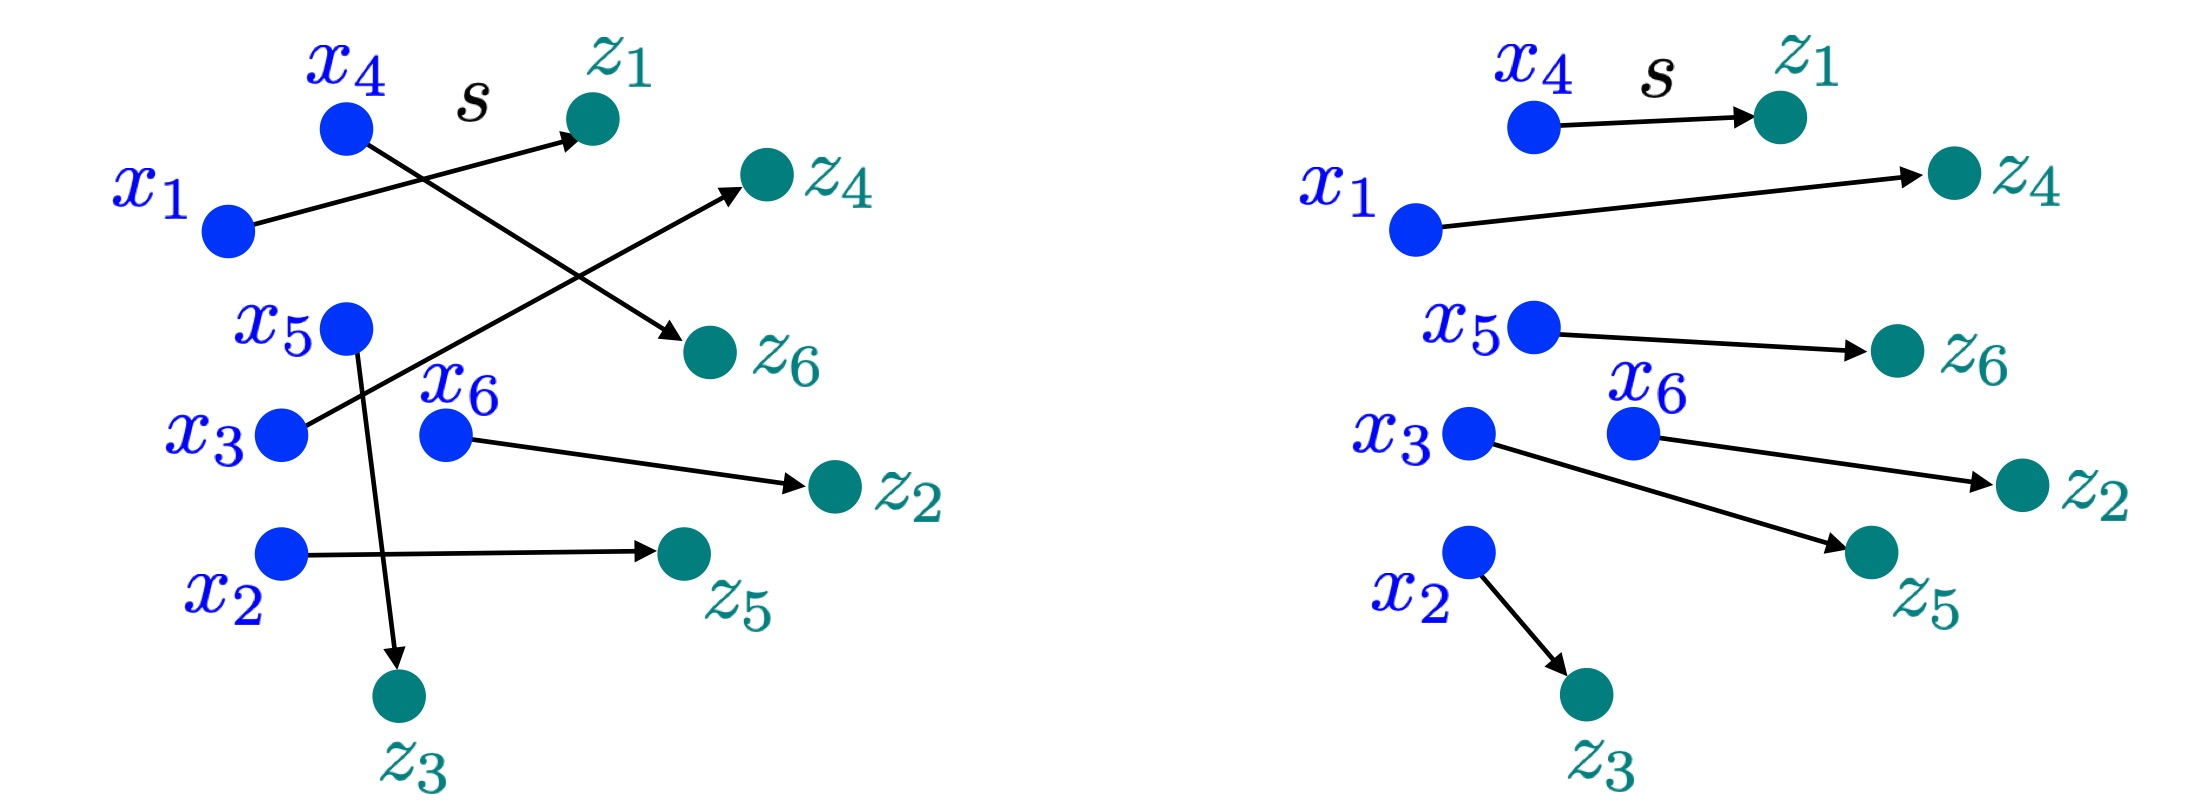
\includegraphics[width=.8\linewidth]{otmonge.jpg}
\caption{\label{fig:otmonge} Exemple à gauche d'une permutation $s$ non-optimale et à droite de la permutation optimale, dans le cas de $6$ points en dimension 2.  }
\end{figure}

La difficulté pour calculer cette distance est que le nombre total de permutations à tester est très grand. En effet, pour le choix de $\perm{1}$ il y a $n$ possibilités, pour celui de $\perm{2}$ il en y a $n-1$ (puisque la valeur de $\perm{1}$ est prise), pour $\perm{2}$ il y en a $n-2$, etc. Donc le nombre total de permutations est égal à $n!$, la factorielle du nombre $n$, qui est définie comme
\eq{
	n! = n \times (n-1) \times (n-2) \times \ldots \times 2 \times 1.
}
Pour $n=6$ comme à la figure~\ref{fig:otmonge}, il y a donc 
\eq{
	6!=6 \times 5 \times 4 \times 3 \times 2 \times 1 = 720 \text{ permutations possibles.}
}
Dans ce cas simple, on peut toutes les tester et choisir la meilleure, qui est, comme montré à la droite de la figure~\ref{fig:otmonge}, 
\eq{
	(\perm{\myblue{1}}=\mylblue{4},
	\perm{\myblue{2}}=\mylblue{3},
	\perm{\myblue{3}}=\mylblue{5},
	\perm{\myblue{4}}=\mylblue{1},
	\perm{\myblue{5}}=\mylblue{6},
	\perm{\myblue{6}}=\mylblue{2}).
}
La difficulté est que pour $n=70$, il y a plus de $10^{100}$ possibilités, ce qui est à comparer aux $10^{79}$ atomes dans l'univers \ldots Et pour entrainer des réseaux de neurones, $n$ est encore beaucoup plus grand ! 
%
Il a donc fallu attendre plusieurs révolutions mathématiques et algorithmiques pour pouvoir obtenir une méthode permettant de résoudre ce problème. 


%%%%%%%%%%%%%%%%%%%%%%%%%%%%%%%%%%%%%%%%%%%%%%%%%%%%%%%%%%
\section{Le transport optimal de Kantorovitch}
\label{sec-kanto}

Monge a remarqué que les solutions de son problème ont des structures très particulières. Par exemple, on peut observer sur la figure~\ref{fig:otmonge}, à droite, que les trajets optimaux ne se croisent pas, et Monge l'avait prouvé dans son article~\cite{Monge1781}. Mais ceci n'est pas suffisant pour résoudre le problème, car il existe encore énormément de trajectoires sans croisement. Il a fallu plus de 200 ans pour comprendre comment obtenir plus d'information sur les solutions afin de les calculer efficacement. 
%
C'est Leonid Kantorovitch qui a trouvé en, 1942~\cite{Kantorovich42}, une nouvelle formulation du problème de transport optimal calculable rapidement. Il a autorisé chaque source à se diviser en plusieurs parties, par exemple deux parties égales avec une pondération de 1/2 chacune. Cette division de la production est intéressante car elle simplifie le problème d'optimisation. Elle est également naturelle pour les préoccupations de Kantorovitch qui était de modéliser et planifier la production en économie. Il a d'ailleurs obtenu le prix Nobel d'économie pour cette idée. 
%
Conjointement à ces travaux pionniers de Kantorovitch, George Dantzig a trouvé en 1947 l'algorithme du simplexe~\cite{dantzig1990origins}, qui permet de résoudre efficacement des problèmes de transport de grande taille. Sa complexité numérique pour résoudre un problème de transport optimal entre $n$ points est de l'ordre de $n^3 = n \times n \times n$, ce qui est beaucoup plus faible que $n!=n \times (n-1) \times \ldots \times 2 \times 1$. Il est au c\oe{}ur d'un très grand nombre de systèmes industriels qui doivent optimiser l'adéquation entre des moyens de production et de consommation. Et on peut du coup également l'utiliser pour entrainer des réseaux de neurones génératifs ! On pourra regarder~\cite{PeyreCuturi} pour plus de détails sur la théorie du transport optimal, les algorithmes efficaces et ses applications à la science des données. 


%%%%%%%%%%%%%%%%%%%%%%%%%%%%%%%%%%%%%%%%%%%%%%%%%%%%%%%%%%
\section{Les réseaux antagonistes}

Une difficulté pour appliquer le transport optimal pour entrainer des réseaux génératifs est qu'il faut choisir le coût de transport entre deux images. 
%
On pourrait calculer la distance euclidienne entre les pixels des images, mais ceci ne marche pas bien, car cela ne prend pas en compte la géométrie des objets présents dans les images.
%
Une idée très fructueuse a été introduite en 2014 par Ian Goodfellow et ses collaborateurs~\cite{goodfellow2014generative}. Elle consiste à utiliser un second réseau de neurones pour déterminer ce coût de transport~\cite{martin2017wasserstein}. 
%
Ce second réseau $f$, nommé réseau adversaire, joue un rôle de discriminateur. Alors que le but du générateur $g$ est de générer des images fausses très ressemblantes, le but de $f$ est au contraire de faire de son mieux pour reconnaitre les vraies et les fausses images. Ces deux réseaux sont entrainés conjointement, c'est pour cela que l'on parle de réseaux antagonistes.
%
L'entrainement de ces deux réseaux correspond à ce que l'on appelle un jeu à somme nulle, introduit par John Von Neumann en 1944~\cite{morgenstern1953theory} et généralisé ensuite par John Nash en 1950~\cite{nash1950equilibrium}, qui a obtenu tout comme Kantorovitch le prix Nobel d'économie. 

Ces avancées récentes~\cite{goodfellow2014generative} ont ainsi permis d'obtenir des résultats excellents pour la génération d'images. 
%
La figure~\ref{fig:deepfake} montre des résultats obtenus avec la méthode expliquée dans~\cite{brock2018large} et son utilisation pour calculer des \guill{chemins} d'images entre chiens et chats. 

\begin{figure}\centering
	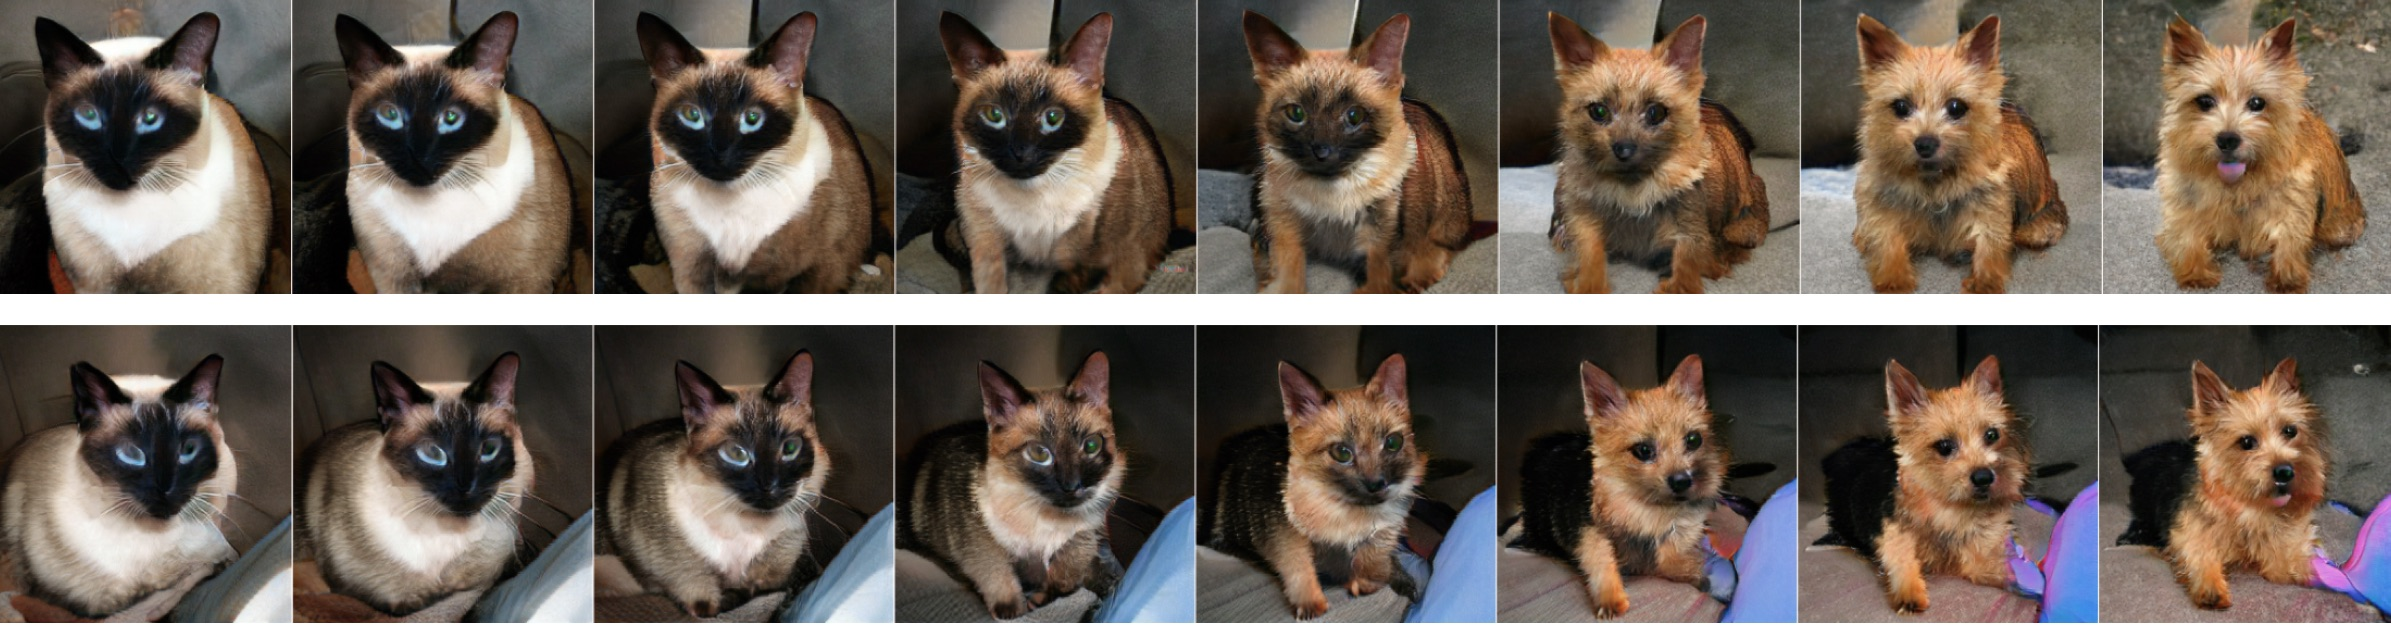
\includegraphics[width=.95\linewidth]{deepfake}
\caption{\label{fig:deepfake} Deux exemples de \guill{deep fakes} qui sont des images virtuelles interpolant entre chats et chiens. }
\end{figure}




\section*{Remerciements}

Je remercie Gwenn Guichaoua pour sa relecture attentive, ainsi que Sébastien Racanière et Vincent Barra pour leurs corrections.

\bibliographystyle{plain}
\bibliography{biblio-nn}

\end{document}

